%----------------------------------------------------------------------------------------
%	PACKAGES AND OTHER DOCUMENT CONFIGURATIONS
%----------------------------------------------------------------------------------------

\documentclass[12pt]{article} % Default font size is 12pt, it can be changed here

\usepackage{geometry} % Required to change the page size to A4
\geometry{a4paper} % Set the page size to be A4 as opposed to the default US Letter

\usepackage{graphicx} % Required for including pictures

\usepackage{hyperref} % Required for hyperlinks

\usepackage{float} % Allows putting an [H] in \begin{figure} to specify the exact location of the figure

\linespread{1.2} % Line spacing

%\setlength\parindent{0pt} % Uncomment to remove all indentation from paragraphs

\graphicspath{{Pictures/}} % Specifies the directory where pictures are stored

\begin{document}

%----------------------------------------------------------------------------------------
%	TITLE PAGE
%----------------------------------------------------------------------------------------

\begin{titlepage}

\newcommand{\HRule}{\rule{\linewidth}{0.5mm}} % Defines a new command for the horizontal lines, change thickness here

\center % Center everything on the page

\textsc{\LARGE University of Auckland}\\[1.5cm] % Name of your university/college
\textsc{\Large COMPSCI 765}\\[0.5cm] % Major heading such as course name
\textsc{\large Interactive Cognitive Systems}\\[0.5cm] % Minor heading such as course title

\HRule \\[0.4cm]
{ \huge \bfseries Multi-Agent Mafia}\\[0.4cm] % Title of your document
\HRule \\[1.5cm]

\begin{minipage}{0.4\textwidth}
\begin{flushleft} \large
\emph{Author:}\\
Bradley \textsc{Moorfield}\\
Sebastian \textsc{Cram}\\
Derek \textsc{Galea}\\
\end{flushleft}
\end{minipage}
~
\begin{minipage}{0.4\textwidth}
\begin{flushright} \large
\emph{UPI:}\\
bmoo063\\
scra069\\
dgal061\\
\end{flushright}
\end{minipage}\\[4cm]

{\large \today}\\[3cm] % Date, change the \today to a set date if you want to be precise

%\includegraphics{Logo}\\[1cm] % Include a department/university logo - this will require the graphicx package

\vfill % Fill the rest of the page with whitespace

\end{titlepage}

%----------------------------------------------------------------------------------------
%	TABLE OF CONTENTS
%----------------------------------------------------------------------------------------

\tableofcontents 
\newpage  

%----------------------------------------------------------------------------------------
%	INTRODUCTION
%----------------------------------------------------------------------------------------

\section{Introduction} 

%------------------------------------------------

\subsection{Overview} 

Mafia~\cite{PRI2015} is a social party game where an informed minority, the mafia, conflicts with an uninformed majority, the innocents. The game is typically played with seven to ten players, with two to three mafia for best results. Many variations on the rules exist, but the basic game focuses on the village as a whole debating the identities of the mafia and voting on one player to lynch during the day, with the mafia choosing one player to kill during the night. The game ends when all the mafia have been eliminated, or the mafia outnumber the innocents. Outside of these rules, the players may do anything to try convince the other players of their innocence, or accuse another player of being mafia. 

Other roles can be assigned, including a medic and a sheriff. The medic has an opportunity during the night to select one individual to be saved, should they be targeted by the mafia. The sheriff has an opportunity during the night to select one individual and be informed by the game master whether that person is mafia or not. 
 
The game master controls the flow of the game and decides when to advance the game onto the next phase. They request the individuals with a particular role to take action at the appropriate time and announce the results of the night’s activities. The game master simply applies the rules of the game, so their actions will be coded in as rules based on the game state. 

The other players will not have full knowledge of the game state, so they will form beliefs about the other agents playing the game. They will have beliefs about their own and others’ roles in the game. They can observe the other agents actions in the game and form beliefs based on those observations. Some basic actions include making an accusation, asking others about their beliefs and making claims about their role in the game. To give them some way to assess the truthfulness of other agent’s claims we may include unintentional actions like a wavering voice, hesitation or perspiration. So there would be same chance if an agent lies about their role, they do so in a wavering voice. For example, one agent accuses another of being mafia. The accused claims they are the medic and perspires. The accuser then forms the belief that they are mafia, as do the other agents. Then when the vote is called they are likely to lynch them. 

One potential way to make the inferences about agents roles more complex is to give the agents some rudimentary personality. Then if the accuser believes the accused is a shy person there is a competing explanation for their perspiration. Other relevant personality traits would be aggressiveness and honesty. These traits would influence how often they make accusations or lie. 



%------------------------------------------------

\begin{figure}[H] 
\center{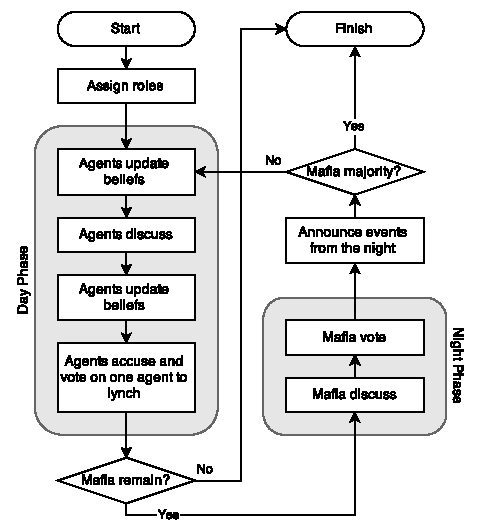
\includegraphics[width=0.75\linewidth]{flow.pdf}}
\caption{Flow chart diagram of Game master}
\end{figure}

%------------------------------------------------

\subsection{Motivation} 

Mafia allows for a variety of challenges from mathematical, computational, and cognitive standpoints. Braverman et al.~\cite{BRA2008} shows extensive mathematical modelling can be applied to even a simple environment. Computationally it follows from from the likes of the Facade and Versu systems in having a simulated set of agents interacting with a user in order to tell a story. The simulated agents also need to interact with each other, as each agent is independent. 

Haan et al.~\cite{HAA2004} have previously implemented a simple mafia playing agent to demonstrate their multi-agent framework, however little reasoning of other agents true beliefs was performed. Our goal is for agents (both real and simulated) to be able to make inferences as to the true status of other agents based on individual announcements and other observables, and perhaps uniquely it requires agents to lie and identify the lies of others. This is a cognitively demanding task, so it will be interesting to see if we can find ways to make the agents intelligently deceptive. 

%------------------------------------------------

\begin{figure}[H] 
\center{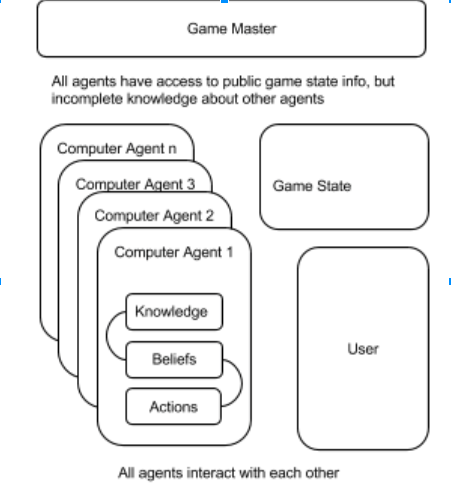
\includegraphics[width=0.6\linewidth]{Entitydiagram}}
\caption{Entity diagram for Multi-Agent Mafia system}
\end{figure}

%----------------------------------------------------------------------------------------
%	Analysis
%----------------------------------------------------------------------------------------

\section{Analysis}

The game starts with the game master assigning roles randomly to all of the players. The game master initiates a discussion phase, then begins the first night phase. The game master first asks the mafia to decide together who to assassinate. Then the medic is called on to select someone to save. Then the sheriff is called on to investigate one player. The game master announces the results of the night and assesses whether the game end conditions are met. Agents update their knowledge and beliefs based on the results. The game master then moves the game into the discussion phase. Agents can make announcements about their beliefs or ask others about their beliefs. To ensure discussions don’t go on forever we can limit each agent to two speech actions (this is a problem in real life games and the game master has to exercise judgement about when to terminate discussions). The game master then moves the game into the accusation phase. Each agent can accuse up to two other people. The game master then allows the accused to defend themselves. They may make claims about themselves or a belief about another player. For example, “I am the sheriff, and I know Bob is mafia” or just deny the accusation or remain silent. Then each player casts their vote publically. 

From information about who voted to lynch, inferences can be made, so knowledge about how people voted should be added to each agent’s knowledge base. For example, if one player made an accusation and claimed they were the sheriff and knew the accused was mafia, a vote is taken and the accused is lynched and they turned out to only be a citizen, the accuser was lying. This may lead players to conclude the accuser is mafia. 

The game master again assesses whether the game end conditions are met. If not, another round of discussion takes place. Then another night falls and the night cycle repeats until one team has won.

%----------------------------------------------------------------------------------------
%	Design
%----------------------------------------------------------------------------------------

\section{Design}

\subsection{Overall Architecture}

Our system is implemented using the Jason Multi-Agent System~\cite{JAS2015}, which provides a framework that allows multiple agents to run simultaneously using a logic-programming BDI language called AgentSpeak~\cite{RAO1996}, communicate with each other, and modify the underlying architecture of agents and the environment.

AgentSpeak encodes agents as a set of beliefs and plans. Beliefs are first-order predicates that define the knowledge of the world as the agent knows it. Plans consist of an event trigger (either the addition or deletion of a belief), a context defined as the conjugation of beliefs, and a sequence of actions that the agent has to achieve when a plan is chosen for execution.

The extended implementation of AgentSpeak used in Jason provides two important internal actions: broadcast and sent. These actions allow an agent to either broadcast a message to all other agents, or send a message to a specific agent. Messages consist of an illocutionary force, a sender, a reciever, and a belief literal. Agents communicate their beliefs by broadcasting their accusations and denials to all, or participate in the game by sending their votes to the game controller.

The overall structure of the system is shown in figure~\ref{fig:overallarch}. The Jason interpreter is responsible for distributing messages from a broadcast or send, so all agents interact with each other through this central hub. In this implementation, the game controller is implemented as an agent that does no reasoning, it simply acts as a man in the middle to intercept communication and keep track of the game.

The game controller has a modified agent architecture. This is a feature of Jason whereby we can write Java code that changes how the agent deals with receiving beliefs, in this case it keeps track of the state of the game, and counts votes that are sent by other agents. The game controller is also able to send out beliefs that tell the agents when the state of the game changes, this happens when the user presses the 'next state' button on the interface presented by the game controller.

The final piece of the puzzle, the user, interacts through the game controller interface. The interface consists of buttons that allow the user to perform actions similar to those that the agents can perform, such as accusing, denying, voting during the town vote or voting during the mafia decision. The buttons become enabled and disabled depending on the state of the game and whether or not the human agent is still alive. The game controller broadcasts messages on behalf of the user whenever the user presses the button for a corresponding action.

\begin{figure}
	\centering
	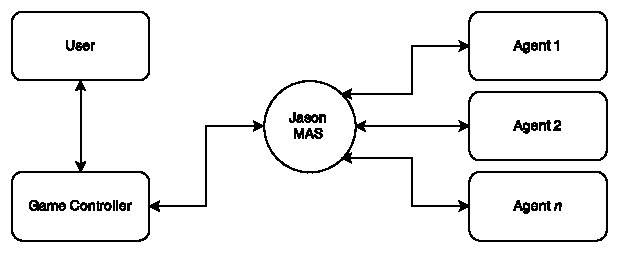
\includegraphics[width=\linewidth]{Overall.pdf}
	\caption{Overall architecture of the Multi-Agent Mafia system}
	\label{fig:overallarch}
\end{figure}

\subsection{User Modelling}

User modelling is quite simple in our system. Every public interaction made during the game is stored in the belief base of all agents, these include accusations, denials, who voted for who during town voting, who was lynched and who died at the hands of the mafia. These beliefs are used in the context of plans to update knowledge on who the agent believes is mafia (or who is a target to kill if the agent is mafia themself).


\subsection{Planning Logic}

Jason and AgentSpeak provide powerful constructs for adding goals, which manifest as desires in BDI terminoligy. These goals or desires can be used to allow an agent to plan out in the long term a 'strategy' to use, such as focusing on convincing a particular agent it isn't mafia. In our implementation we haven't used any of these long term goals, so the agents are only reactive and pick the first set of beliefs that satisfies a plan when a plan is executed.

Our system does have some rules that allow it to reason about who is mafia or a target, which encode how an agent plans to vote during voting stages of the game. An example would be a rule that says if agent A accused agent B, and the mafia killed agent A during the night, then agent B was likely an accurate accusation. However mafia can take advantage of this situation too: if A accuses B, B is not mafia, and mafia don't have a particular target to kill, then B could be a good choice to lead villagers astray. This problem is mentioned in the limitations section of our report.

%----------------------------------------------------------------------------------------
%	Practical
%----------------------------------------------------------------------------------------

\section{Practical}

\subsection{Ilustration}

Unlike other systems which may have to work with abstract test cases, the advantage in a game system is that testing is simply done by playing. What follows is a step through what a player would expect to see when playing. 

\begin{figure}[H]
\centering
\begin{minipage}{0.49\textwidth}
\centering
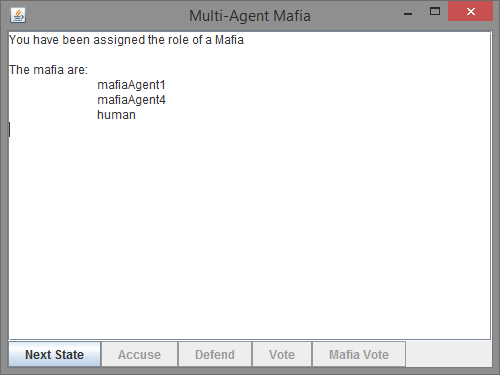
\includegraphics[width=\linewidth]{mafia-start}
\caption{Start State}
\label{fig:start}
\end{minipage}\hfill
\begin{minipage}{0.49\textwidth}
\centering
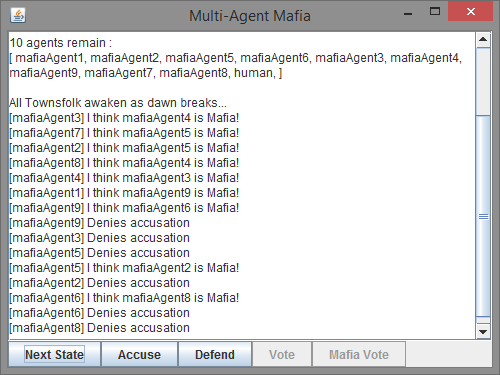
\includegraphics[width=\linewidth]{mafia-discussion}
\caption{First round of accusations}
\label{fig:discussion}
\end{minipage}
\end{figure}

Figure \ref{fig:start} is an example of what appears upon initiation of the system, it allows an agent to see their randomly assigned role and, in the case of mafia, who the other mafia agents are. Figure \ref{fig:discussion} shows what, if anything, each agent publically announces. The actions the player may take in the current implementation are limited to simply accusing another agent, or defending one who has already been accused. Taken to it's extreme this could be accomplished with a natural language interface, this is sufficient as a demonstration of the system.

\begin{figure}[H]
\centering
\begin{minipage}{0.49\textwidth}
\centering
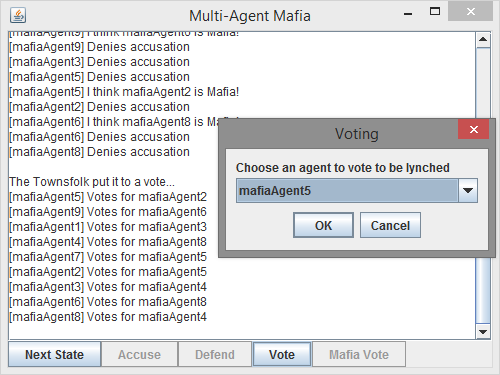
\includegraphics[width=\linewidth]{mafia-townvote}
\caption{All agents voting who to kill}
\label{fig:tvote}
\end{minipage}\hfill
\begin{minipage}{0.49\textwidth}
\centering
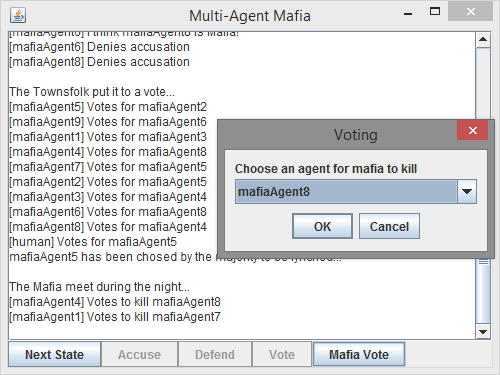
\includegraphics[width=\linewidth]{mafia-mafiavote}
\caption{Mafia agents voting who to kill}
\label{fig:mvote}
\end{minipage}
\end{figure}

From here each agent decides who, if anyone, will be eliminated from the game. Figure \ref{fig:tvote} shows the voting interface. We opted for a simple one agent one vote strategy to allow so quick gameplay, as opposed to interative voting until an absolute majority is reached. This can be explained in game terms as a private vote as opposed to a public one. While the system could be modified there is little reason to at this point due to limitations on available discourse options. Finally figure \ref{fig:mvote} shows what happens during the night. As opposed to previous steps which everyone sees, these are all private to like typed agents. Again, a simple majority is all that is required for the mafia. A villager on the other hand simply sleeps through the night (although some don't wake up).

\subsection{Limitations}

There are four key components which could further be implemented. Those being roles, personality, memory, and discourse.

\subsubsection{Roles}
We only implemented the simplest roles required to form a coherent game, those being villagers and mafia. There are other roles that could be assigned however. These include the doctor who, after the mafia has selected a victim, is allowed to choose one person to live through the night, and the sheriff who once each night can consult the system for the role of another agent.

\subsubsection{Personality}
Each agent within the system is presently homogeneous. With further development we could see the agents gaining their own seperate attribtes and personalities. For instance one agent could be partiularly charismatic allowing other agents to be more easily convinced by their accusations. Two agents could perhaps feud, leading them to often accuse each othe regardless of plausability. Individual agents may also have tells, such as a stutter or becoming flush, indicating they may be lying.


\subsubsection{Memory}
At present each game takes place in isolation. Further implementation would perhaps allow for a continued memory for the agents. Allowing for grudges that last between games, and forming opinions on the honesty and charisma of other agents.

\subsubsection{Discourse}
In it's simplest form we implemented only the ability to 'accuse' and 'deny' membership of the mafia. While a full natural language interface might be achievable, we would focus more on expanding how each of those actions take place. Accusations through inference "agents 1 accused agents 5, now agent 1 is dead" vs passion "agent 3 was mafia last game and they killed me!". Even during the voting stages perhaps being able to defend others to sway certain votes.

\subsection{Demonstration}

A working run playing as a member of the mafia is available
\href{https://www.dropbox.com/s/go9x8617lvtuozv/Mafia%20Demonstration.mp4?dl=0}{here}

%----------------------------------------------------------------------------------------
%	The Team
%----------------------------------------------------------------------------------------

\section{About the Authors}

\subsection{Bradley Moorfield}

Initial planning and development. Program design. Coding. Report copy.

\subsection{Sebastian Cram}

Initial planning and development. Program design. Report copy. Report formatting

\subsection{Derek Galea}

Initial planning and development. Program design.

%----------------------------------------------------------------------------------------
%	MAJOR SECTION X - TEMPLATE - UNCOMMENT AND FILL IN
%----------------------------------------------------------------------------------------

%\section{Content Section}

%\subsection{Subsection 1} % Sub-section

% Content

%\begin{figure}[H] 
%\center{\includegraphics[width=0.5\linewidth]{examplefile}}
%\caption{Example image.}
%\label{fig:speciation}
%\end{figure}

%------------------------------------------------

%\subsection{Subsection 2} % Sub-section

% Content

%----------------------------------------------------------------------------------------
%	BIBLIOGRAPHY
%----------------------------------------------------------------------------------------
\newpage
\begin{thebibliography}{99} % Bibliography - this is intentionally simple in this template

\bibitem{PRI2015}
The Graduate Mafia Brotherhood of Princeton University
\emph{http://www.princeton.edu/~sucharit/~mafia/}
Accessed March (2015)

\bibitem{BRA2008}
Braverman, M., Etesami, O., Mossel, E. (2008).
Mafia: A Theoretical Study of Players and Coalitions in a Partial Information Environment.
Annals of Applied Probability.

\bibitem{HAA2004}
Haan, H. W. D., Hesselink, W. H., Renardel de Lavalette, G. R. (2004).
An abstract multi-agent framework applied to a social interaction game.
University of Groningen, Johann Bernoulli Institute for Mathematics and Computer Science.

\bibitem{JAS2015}
Jason
\emph{http://sourceforge.net/projects/jason/}
Accessed April (2015)

\bibitem{RAO1996}
Rao, A. (1996).
AgentSpeak(:): BDI agents speak out in a logical computable language.
Lecture Notes in Artificial Intelligence.
 
\end{thebibliography}

%----------------------------------------------------------------------------------------

\end{document}
